\newpage
\subsection{PQR}

\textbf{Motivation.} During the initial research for a thesis subject, I came across \cite{dlchess:2014} which seemed an interesting approach to train a neural network to evaluate positions. Since it was released in 2014, it predates the NNUE era and the training data was suboptimal (Lichess database \cite{lichessdb} with human moves). So I decided to try to replicate the idea using modern datasets, better moves and a proper engine. The \enquote{PQR} method itself was explained in detail in the previous chapter.  Remember that $p$ is a position in the dataset, $q$ is the position obtained by making the best move according to the dataset and $r$ is a random position obtained making a random move from $p$ such that $r \neq q$. \\

Before starting the experiment, I checked if existing networks trained with the conventional method behave under the principles of the PQR method: ${f(p) = -f(q)}$ and ${f(r) > f(q)}$. In the left plot of figure \ref{pqr-eval}, we can see that values of $f(p)$ and $f(q)$ are negatively correlated, which supports the principle that $f(p)=-f(q)$. In the right plot, we can see that the distribution of the difference between $f(r)$ and $f(q)$ is mostly positive, which supports the principle that $f(r) > f(q)$. This shows that the principles that the PQR method relies on are properties that manifest in existing models.

\begin{figure}[H]
\centering
\makebox[\textwidth]{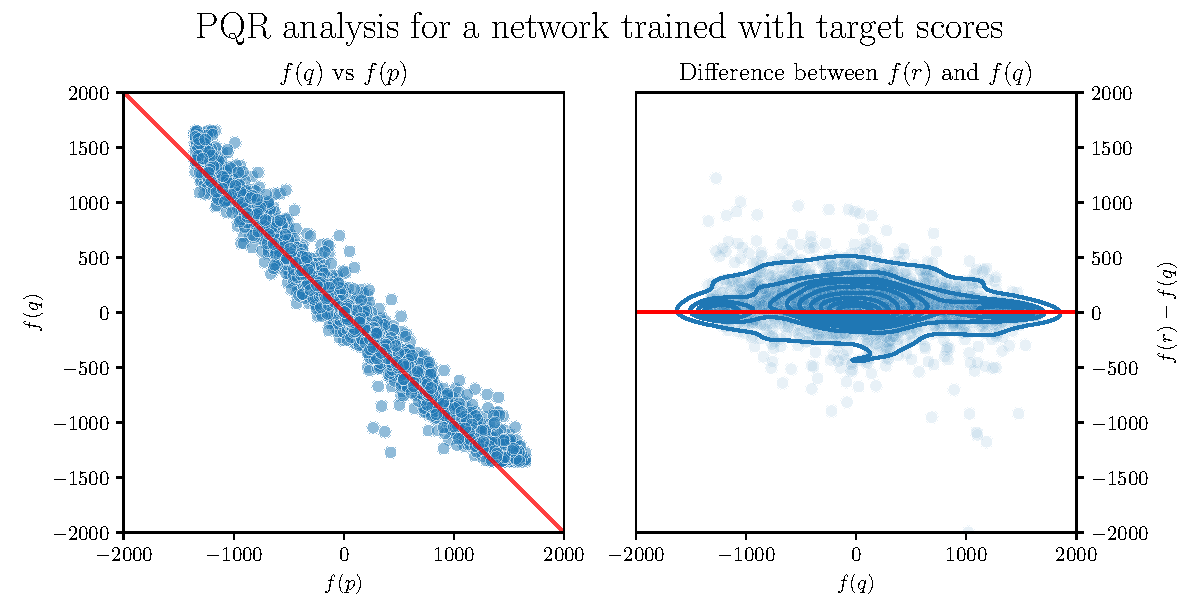
\includegraphics[width=\textwidth]{./dynamic/output/pqr_eval.pdf}}
\caption{Analysis of $N=4000$ PQR samples using a model trained with target scores and the feature set \featureset{All}.}
\label{pqr-eval}
\end{figure}

\newpage
\textbf{Experiment.} I will train the canonical \featureset{All} feature set with this method in two ways:

\begin{enumerate}[label=\bf\Alph*.]
\item \textbf{Train from scratch.} The network is initialized with random weights and trained with the PQR method. This is what the original authors did, and I do not expect to reach the performance of models trained with the evaluations method. Using precomputed evaluations as a target is a lot simpler for the model, since it only has to learn to mimic the scores.

\item \textbf{Continue from a checkpoint.} A strong checkpoint trained with the other method is used to initialize the network. This way, the network does not have to learn too much at once and may enable it to improve the existing parameters. I believe that two scenarios are likely to happen: the model improves very slowly, or it completely forgets what it have learned before and ends up like a model trained from scratch. The best scenario is that the model improves slowly, proving that it can be used to further optimize existing models.
\end{enumerate}

The training data is not filtered the same way as with target scores, where it was known that captures and checks are detrimental. When choosing a random position $R$ from a position $P$, the number of available moves to choose from is $m$ (including $P \rightarrow Q$). A training sample is skipped if $m < M$. The reasoning behind $M$ is that the bigger the pool to choose from, the more likely it is to find a move that is worse than $P \rightarrow Q$. Note that $M \geq 2$ since otherwise there is only one available move.

Choosing fixed values of $M$ is not ideal, since the number of available moves varies throughout the game. A value of $M$ will be chosen for every turn in the game, based on the distribution of available moves for that particular turn and color. It is known that the white player has more available moves in average than the black player, so $M$ will be different for each.

Four networks will be trained from scratch where $M$ is chosen to filter 0\%, 25\%, 50\% and 75\% of samples with the least available moves for that turn. In figure \ref{avg-moves} we can see the value of $M$ changing throughout the game for each quantile. Note that when $p=0$, $M=2$ in every turn, so no filtering is done. \\

\begin{figure}[H]
\centering
\makebox[\textwidth]{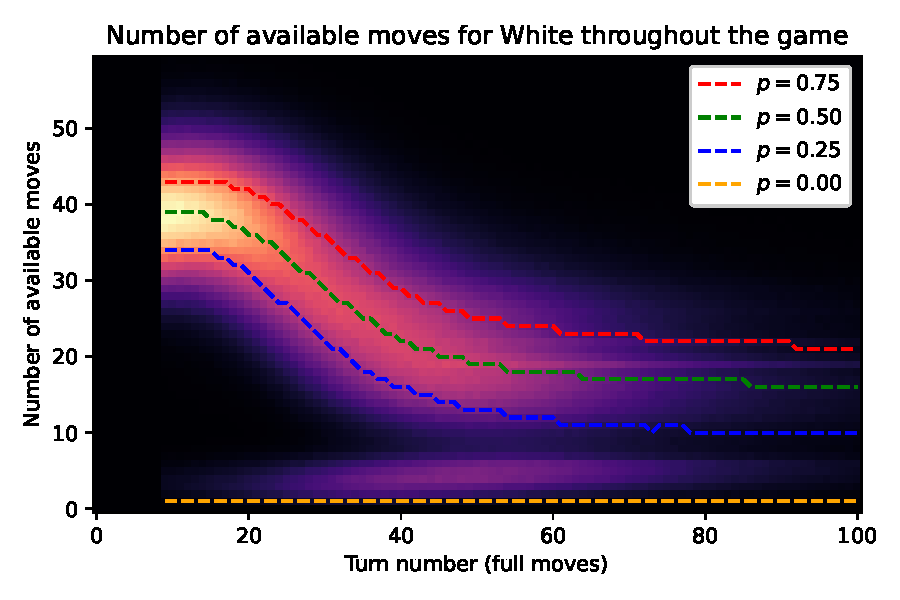
\includegraphics[width=\textwidth]{./dynamic/output/avg_moves.pdf}}
\caption{Heatmap showing the number of available moves for white throughout 100 turns (full moves). The color gradient indicates the density of occurrences in the dataset (N=25M) for positions with a certain number of available moves in a given turn. The plot for black is not shown because it is very similar. The dataset provides positions that start at turn 9.}
\label{avg-moves}
\end{figure}

\newpage
\textbf{(A) Results.} The networks are able to learn with the PQR method from scratch, without the use of existing evaluations like the other method. In figure \ref{pqr-evolution}, we can see the evolution of the ratings of each of the networks trained, along with a network trained with target scores.

\begin{figure}[H]
\centering
\makebox[\textwidth]{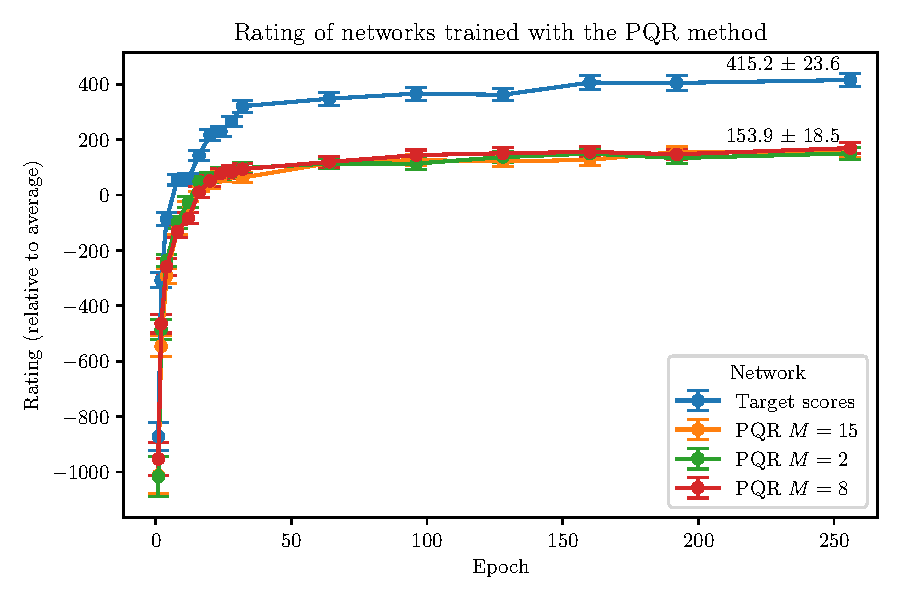
\includegraphics[width=\textwidth]{./dynamic/output/pqr_comparison.pdf}}
\caption{Performance of networks trained from scratch using the PQR method varying the filtering parameter ($p=0,\ 0.25,\ 0.5,\ 0.75$). A network trained with target scores is shown for comparison.}
\label{pqr-evolution}
\end{figure}

The target scores method outperforms the best PQR network by $235 \pm 41$ rating. This result was anticipated, since the target scores method is a lot simpler for the network to learn.

Contrary to what was expected, the larger the pool of moves to choose from (higher values of $p$), the worse the network performs. It was expected that with a higher $M$, it was more likely to find a move that was worse than $P \rightarrow Q$, but this was not the case. A possible explanation is that the positions located in the bottom cloud of the distribution in figure \ref{avg-moves} are good training samples for this method. In the other method, this positions were excluded since most are check positions. The experiment was run again including check positions but the results were the same. \\

\newpage
When looking at the behaviour of $f$ in figure \ref{pqr-scratch}, it does resemble what we expect to happen, a negative correlation between $f(p)$ and $f(q)$ and a positive difference between $f(r)$ and $f(q)$. However, the correlation is a lot more spread out, specially in $f(p)=-f(q)$, which is crucial that they are as close as possible since the network would be predicting different scores for the same position but the other perspective.

A possible improvement could be to try to increase the weight of the $f(p)=-f(q)$ inequalities in the loss function, to force the network to be more like the target scores method. This means reducing the spread in the left plot and give less importance to high differences of $f(r)-f(q)$ since the values should not be as extreme. This is left for future work.

\begin{figure}[H]
\centering
\makebox[\textwidth]{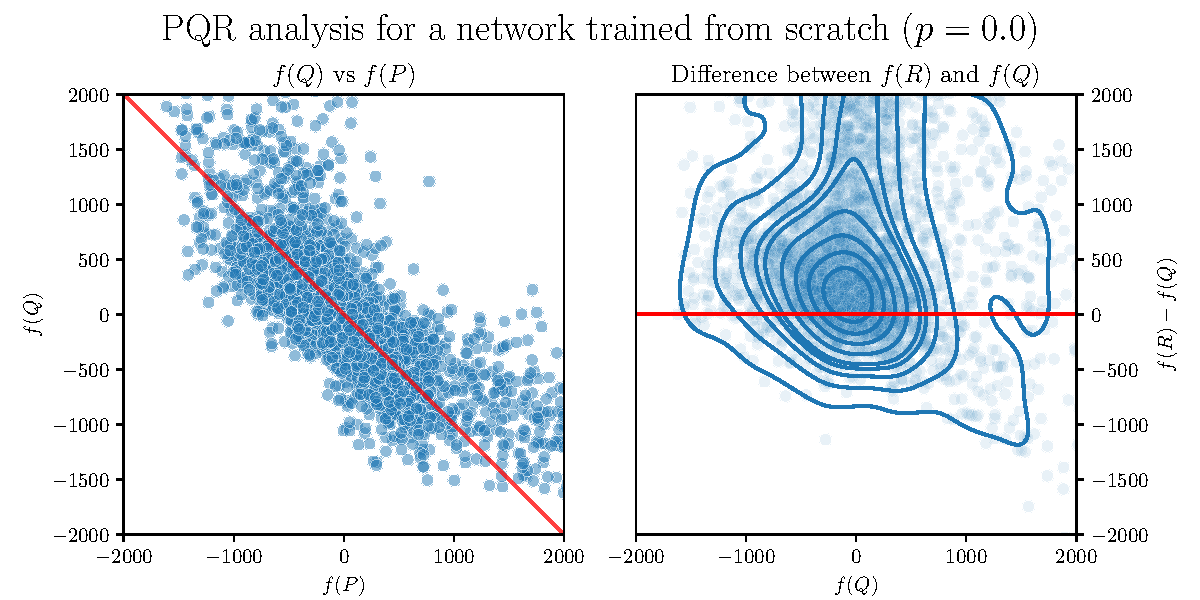
\includegraphics[width=\textwidth]{./dynamic/output/pqr_scratch.pdf}}
\caption{Analysis of $N=4000$ PQR samples using the epoch 256 of the model trained from scratch with no filtering ($p=0.0$) and the feature set \featureset{All}.}
\label{pqr-scratch}
\end{figure}

Of course everything boils down to the dataset, and the dataset used is not ideal for PQR. There are no guarantees that the $P \rightarrow R$ move is not similar in strength or in fact worse than $P \rightarrow Q$. Not only that, but the scale is not the same for all samples. Positions that have a small but significant difference in strength are being penalized the same way as more extreme ones. Trying filter by the number of available moves did not work, so there is no way around it. \\

A good dataset for PQR can be generated using multiple lines of play (maybe dozens), and only include samples where there is a significant difference in strength between the $P \rightarrow Q$ and $P \rightarrow R$ moves. This also can prevent zugzwang\footnote{A zugzwang position occurs when any move a player can make, worsens their position.} positions from being included. It is necessary to decide what threshold is considered significant. One may analyze the distribution of differences and find something good, but in the end we are trying to convey this information to the network, which is what target scores already does, and better. \\

\textbf{(B) Results.} The checkpoint used to continue training is the epoch 256 of the network trained with target scores that appear in figure \ref{pqr-evolution} (rightest purple dot). The training was done for four different values of learning rate: $0.0005$ (previous initializer), $0.0003$, $0.0001$ and $0.00005$. Different values were used to make sure the network does not forget "too fast" what it has learned before. The results are shown in figure \ref{pqr-ckp}.

\begin{figure}[H]
\centering
\makebox[\textwidth]{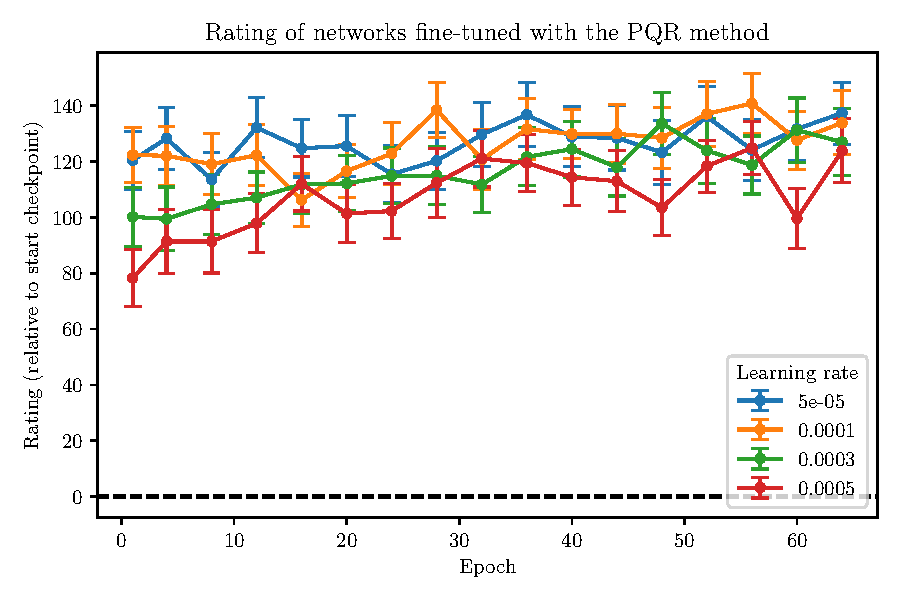
\includegraphics[width=\textwidth]{./dynamic/output/pqr_ckp.pdf}}
\caption{Performance of networks fine-tuned with the PQR method, starting from a target scores checkpoint. The dotted line represents the rating of the checkpoint, which all ratings are relative to.}
\label{pqr-ckp}
\end{figure}

There are a few things to notice in this graph. First, there is a sudden jump from the checkpoint to the first epoch. Since the checkpoint is the starting point, all networks jump in the first epoch to +100 rating.

- sudden jump
- lower LR better
- upwards trend